\Aufgabe[e]{Integrale in $\mathbb R^3$}{
Man betrachte die Kugel
$$K := \left\{ (x,y,z)^{\top} \in \mathbb{R}^3 \mid x^2+y^2+z^2 \leq 4\right\}.$$
Das Volume des Zylinders $$Z := \left\{ (x,y,z)^{\top} \in \mathbb{R}^3 \mid x^2+y^2 \leq 1\right\}$$ wird von der Kugel abgezogen. Bestimmen Sie das Volumen des resultierenden Körpers.

\vspace{1ex}
Hinweis: Man verwendet Zylinderkoordinaten. Das Volumen einer Kugel mit dem Radius $R$ ist $\displaystyle \frac{4}{3}\pi R^3$.
\begin{figure}[h!]
\centering
\begin{tabular}{cc}
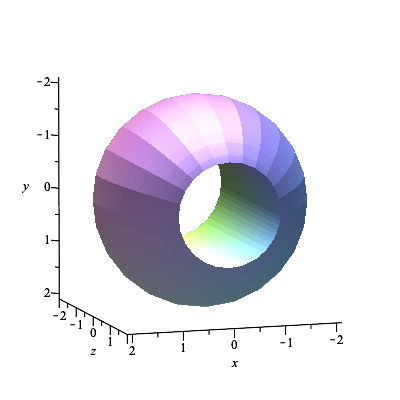
\includegraphics[width=0.5\linewidth]{../A/Wiederholung/figex3b.png}&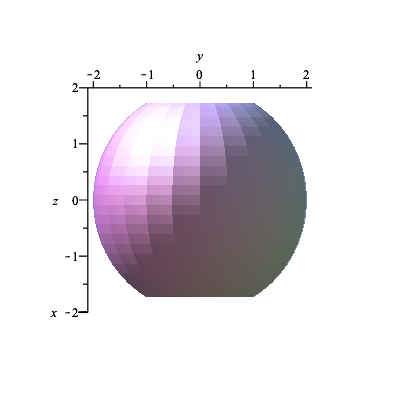
\includegraphics[width=0.5\linewidth]{../A/Wiederholung/figex3a.png}
\end{tabular}
\end{figure}
}

\Loesung{
Wir berechnen zunächst das Volumen des extrahierten Zylinders über der Ebene $(x,y)$, bezeichnet mit $G$. Dazu verwenden wir die zylindrischen Koordinaten und die entsprechenden Transformationen
$$
\begin{pmatrix}
 x\\y\\z
\end{pmatrix}
=
\begin{pmatrix}
 r \cos(\varphi)\\ r \sin(\varphi)\\ z
\end{pmatrix}.
$$
wobei $r \in [0,1],\ \varphi \in [0, 2\pi)$ und da wir nur das Volumen oberhalb der $(x,y)$-Ebene berechnen, $z\geq 0$. Die obere Grenze für $z$ wird aus der Kugelgleichung wie folgt berechnet:
\begin{eqnarray*}
x^2+y^2+z^2 &\leq &4 \\
r^2 + z ^2 &\leq &4 \\
z &\leq& \sqrt{4 - r^2} 
\end{eqnarray*}
Daraus folgt,
$$
G = \left\{
(r,\varphi,z) : 1 \leq r \leq 2,\ 0 \leq \varphi \leq 2
\pi,\ 0 \leq z \leq \sqrt{4 - r^2} \right\}.
$$
Das Volumen wird durch Integration des Volumenelements in zylindrischen Koordinaten wie folgt berechnet
\begin{eqnarray*}
\iiint\limits_{G} r \, \mathrm{d}r \, \mathrm{d}\varphi \, \mathrm{d}z &=&
 \int \limits_{0}^{2 \pi} \int \limits^{2}_{1}  \int \limits_{0}^{\sqrt{4-r^2}}
r \, \mathrm{d}z \, \mathrm{d}r \, \mathrm{d}\varphi   
= \int\limits_{0}^{2 \pi} \int\limits^{2}_{1} r \int \limits_{0}^{\sqrt{4-r^2}}
 \, \mathrm{d}z \, \mathrm{d}\varphi \, \mathrm{d}r \, \\\
&= &\int\limits_{0}^{2\pi} \int\limits_{1}^{2} r \sqrt{4 - r^2} \, \mathrm{d}r
\, \mathrm{d}\varphi \overset{t:=4-r^2}{=} \int\limits_{0}^{2\pi} -\frac12 \int\limits_{3}^{0} \sqrt{t} \, \mathrm{d}t \, \mathrm{d}\varphi \\\ 
&= & 2 \pi \sqrt{3}.
\end{eqnarray*}
Das Volumen der Kugel nach Abzug des Zylinders $Z$ ist das Integral mal zwei, weil wir nur den oberen Teil des Körpers integriert haben
$$
K \setminus Z = 4 \sqrt{3} \pi.
$$


\rule{360pt}{1pt}
\cleardoublepage
}
